\section{Röntgenfluoreszenz}
Wird ein Atom durch die Absorption eines Röntgenphotons ionisiert, sodass ein Elektron aus einer inneren Schale mit dem Energieniveau $E_k$ das Atom verlässt, so kann ein beliebiges Elektron des Atoms mit der Energie $E_i > E_k$ in den freien Zustand zurückfallen, insofern dieser Übergang erlaubt ist. Dabei wird ein Fluoreszenzphoton gemäß $h \cdot \nu = E_i - E_k$ frei \cite[S.~261]{dem3}.

\begin{figure}[H] 
  \centering
     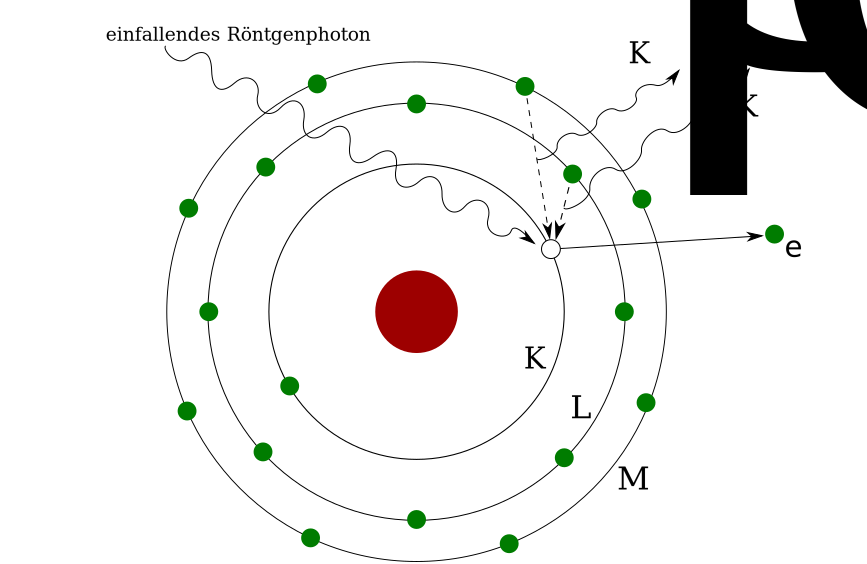
\includegraphics[width=0.65\textwidth]{illustrations/fluorescence.png}
  \caption[Skizze Fluoreszenz]{Die Erzeugung von Fluoreszenzphotonen durch vorherige Anregung mit einem Röntgenphoton ist hier abgebildet. Zur Veranschaulichung sind die Energieniveaus im Bohr'schen Atommodell gezeichnet \cite[S.~25, bearbeitet]{hanna}.}
  \label{fig:fluoreszenz}
\end{figure}

\noindent Wie in \cref{fig:fluoreszenz} dargestellt sind die Fluoreszenzlinien nach den Übergängen benannt. So entsteht beispielsweise ein Photon der $K_{\beta}$-Linie beim Übergang eines Elektrons von der $M$-Schale in die $K$-Schale eines Atoms unter Emission eines Photons der Energie $E_M - E_K$. Die möglichen Energieniveaus der Elektronen eines Atoms sind durch seine Quantenzahlen bestimmt. Diese sind für unterschiedliche Elemente nicht gleich. Daher sind auch die möglichen Energieniveaus der Elektronen nicht gleich. Demzufolge lassen sich die durch Fluoreszenz ausgelösten Elektronen über ihre Energie einem Element zuordnen. Man spricht bei diesem Effekt von charakteristischer Röntgenstrahlung.
